\chapter{Bahnoptimierung}
%\cite{Eggers.2019}
%\cite{Engelke.2008}
%\cite{Ziaukas.2017}
%\cite{Hansen.2012}
%\cite{Spong.2020}
%
\section{Definition des Optimierungsproblems}
Gegenstand der Optimierung ist die Minimierung des Energieverbrauchs eines KR210 R2700-2 Industrieroboters entlang einer Bewegungsbahn. Im Ziel der Arbeit ist festgelegt, den Ansatz möglichst praktikabel für die Automobilproduktion zu gestalten. Dazu wird der Begriff der Bewegungsbahn weiter eingegrenzt. Es wird unterschieden zwischen prozessbezogenen Bewegungen, z.B. entlang einer Schweißnaht oder Klebebahn, und nicht-prozessbezogenen Bewegungen, z.B. das Anfahren einer Vorposition oder der Home-Position in der Bewegungsart PTP. Im Folgenden werden explizit nicht prozessrelevante Trajektorien betrachtet. Der Ansatz basiert auf der geometrischen Anpassung  der Bewegungsbahn durch einen zu optimierenden Parametervektor $\bm{q}_{v}$. Dieser umfasst die Gelenkwinkel des, nach der Hälfte der Bewegungsdauer definierten Via-Punkts \cite[S~532~ f.]{Ziaukas.2017}.
%
\begin{equation}
	\bm{q}_{v} = [q_{v,1},...,q_{v,6}]^T 
\end{equation}
%
Der Startwert jedes Via-Punkts wird auf der Hälfte der Winkelposition zwischen dem Start- und Zielpunkt definiert.
\begin{equation}
	q_{v,i,Start} = \dfrac{q_{s,i}+q_{e,i}}{2}
\end{equation}
Die Minimierung der Leistungsaufnahme basiert auf der konfigurationsabhängigen Reduktion der Massenträgheitsmomente in $\bm{M}(\bm{q})$, so dass bei gleichbleibender Winkelbeschleunigung die Drehmomente in den Gelenken reduziert werden \cite[S.~531]{Ziaukas.2017}. Das Optimierungsproblem besteht darin, den Parametervektor zu identifizieren, für den die minimale Zielfunktion erreicht wird.
%\begin{equation}
%	\bm{q}_{v,opt} = \argminA_{\bm{q}_{v}} J_{P_{zu}}(\bm{q}_{v}).
%\end{equation}
%
\begin{equation}
	\argminA_{\bm{q}_{v}} J(\bm{q}_{v}) = \{\bm{q}_{v} \mid J(\bm{q}_{v}) = \min_{\bm{q}_{v,opt}} J(\bm{q}_{v,opt})\}.
\end{equation}
%
\section{Zielfunktion}
Für die Definition der Zielfunktion wird angenommen, dass die generatorisch erzeugte Leistung während des Abbremsvorgangs über Bremswiderstände dissipiert. Zur Identifizierung des Optimums werden die Zielfunktionen \ref{eqn:torque} \cite[S-~1]{Hansen.2012} und \ref{eqn:emech} \cite[S.~57]{Eggers.2019} aufgestellt. Die Integrationsgrenzen $t_s$ und $t_e$ entsprechen dem Start- bzw. Zielzeitpunkt. Der Ausdruck \ref{eqn:torque} erzielt durch Quadrieren den Vorteil, dass hohe Drehmomente stärker gewichtet werden.
%
\begin{equation}
	\label{eqn:torque}
	J_{\tau}(\bm{q}_{v}) = \frac{1}{2}\int_{ts}^{te}\sum_{i=1}^{n}\left|\tau_i(t)\right|^2~dt
\end{equation}
%
Von einem Vorschlag der Zielfunktion \ref{eqn:emechges} \cite[S.~1216]{Saravanan.2008} wird Abstand genommen, da hierbei die generatorisch umgewandelte Leistung während des Abbremsvorgangs als aufgenommene Leistung der Verbraucher bewertet wird. 
%
\begin{equation}
	\label{eqn:emechges}
	J_{P_{mech_{ges}}}(\bm{q}_{v}) = \int_{ts}^{te}\sum_{i=1}^{n}\left|\tau_i(t)\dot{q_i}\right|^2~dt
\end{equation}
%
Die Zielfunktion \ref{eqn:emech} entspricht dem physikalischen Ausdruck der verrichteten Arbeit mit positiven Vorzeichen. Infolgedessen wird ausschließlich die, motorisch aufgenommene, mechanische Leistung berücksichtigt. 
%
\begin{equation}
	\label{eqn:emech}
	J_{P_{mech_{zu}}}
	(\bm{q}_{v}) 
	= E_{mech_{+}}(\bm{q}_{v}) 
	=\int_{ts}^{te}P_{mech_{zu}}(\bm{q}_{v},t)~dt
\end{equation}
%
Die numerische Implementierung der Zielfunktion in  MATLAB\textsuperscript{\textregistered} entspricht der Gleichung  \ref{eqn:numerischezielfunktion}. Die Schrittweite ist in Anlehnung an die Abtastung der Messeinrichtung  mit $\Delta t = 0.004 \text{s}$ festgelegt. Die Anzahl der Schritte $m$  wird gemäß $(t_s-t_e)/\Delta t$ berechnet.
%
\begin{equation}
	\label{eqn:numerischezielfunktion}
	J_{P_{mech_{zu}}}
	(\bm{q}_{v}) 
	= E_{mech_{+}}(\bm{q}_{v}) 
	= \sum_{k=1}^{m} P_{mech_{zu}}(\bm{q}_{v},t)~\Delta t
\end{equation}
%
\section{Nebenbedingungen}
Die Verfahrzeit bleibt gegenüber der Initialbahn konstant und wird durch den Zielzeitpunkt $t_e$ vorgegeben. 
%Eine Anpassung der Variablen für die maximale relative Geschwindigkeit $vel axis[i]$ und Maximalbeschleunigung $acc axis[i]$ im KRL Programm siehe \cite[S.~532]{Ziaukas.2017} erfolgt nicht.
In \cite[S.~40]{Eggers.2019} bzw. \cite[S.~5]{Hansen.2012} werden die Gelenkwinkel der energieoptimalen Bewegungsbahn in der Robotersteuerung über einen Software-in-the-Loop (SiL) Ansatz berechnet. Dadurch ist die Einhaltung von Drehmoment-, Gelenkwinkel-, Geschwindigkeit- und Beschleunigungsgrenzen entsprechend der Gleichungen \ref{eqn:conpos},\ref{eqn:convel}, \ref{eqn:conacc} und \ref{eqn:contau} gewährleistet. 
%
\begin{equation}
	\label{eqn:conpos}
	q_{i,min} \leq q_{i}(t) \leq q_{i,max}  ~\forall~ i \in \{1,2,3,4,5,6\}
\end{equation}
%
\begin{equation}
	\label{eqn:convel}
	\dot{q}_{i,min} \leq \dot{q}_{i}(t) \leq \dot{q}_{i,max}  ~\forall~ i \in \{1,2,3,4,5,6\}
\end{equation}
%
\begin{equation}
	\label{eqn:conacc}
	\ddot{q}_{i,min} \leq \ddot{q}_{i}(t) \leq \ddot{q}_{i,max}  ~\forall~ i \in \{1,2,3,4,5,6\}
\end{equation}
%
\begin{equation}
	\label{eqn:contau}
	\tau_{i,min} \leq \tau_{i}(t) \leq \tau_{i,max}  ~\forall~ i \in \{1,2,3,4,5,6\}
\end{equation}
%
In der vorliegenden Arbeit sind als Nebenbedingungen ausschließlich die Grenzen der Gelenkwinkel $q_{v,i}$ im Via-Punkt definiert. Die Formulierung zielt darauf ab, dass die optimierte Bewegungsbahn nicht signifikant von der Initialbahn abweicht \cite[S.~5]{Hansen.2012}.
\begin{equation}
	q_{v,i} \in [q_{i,min};q_{i,max}] ~\forall~ i \in \{1,2,3,4,5,6\}
\end{equation}
Grenzwerte für die Drehmomente, Winkelgeschwindigkeiten und Winkelbeschleunigungen werden nicht explizit formuliert.  Im Anschluss an die Optimierung erfolgt eine manuelle Überprüfung der Verläufe.
%
\section{Solver- und Optimierungsalgorithmus}
%todo Solver und Optimierungsalgorithmus
%
\section{Durchführung und Auswertung der Optimierungsergebnisse}
Die Untersuchung verfolgt den Anspruch, dass die identifizierten Einsparungen über das Laborumfeld hinaus in der industriellen Praxis realisiert werden können. Dazu wird eine Bewegung der Bewegungsart PTP betrachtet, die in nahezu jedem Programm den Verfahrweg nach Programmende in die Grundstellung abbildet. Exemplarisch wird die Fahrt vom letzten Prozesspunkt zurück in die Grundstellung im Fertigungsprogramm  $Kleben-Seitenwand$  optimiert. Neben der Energieeinsparung wird auch die Verfahrzeit des Roboters auf der neuen Bewegungsbahn analysiert.
% todo OPtimierungsprocedere
% Auswertung

Die identifizierten, energieoptimalen Via-Punkte sind in der Tabelle \ref{tab:optviapunkte} aufgeführt. Auffällig ist, dass für $q_{v,3}$ und $q_{v,4}$ die obere Grenze aktiv ist, sowie für $q_{v,6}$ die untere Grenze d. h. der Gelenkwinkel im Via-Punkt liegt auf dem selben Wert wie der Gelenkwinkel im Start- bzw. Zielpunkt. Für den Gelenkwinkel $q_{v,5}$ wird festgehalten, dass dieser auffällig nah am unteren Grenzwert liegt. Daraus folgt, dass die berechnete Trajektorie für die Gelenkwinkel drei, vier und sechs Werte außerhalb des Intervalls $[q_{i,s};q_{i,e}] ~\forall~ i \in \{3,4,5,6\}$ annimmt. 
\\
\begin{table}
	\centering
	\begin{tabular}{|l|l|l|}
		\hline
		Startwert Gelenkwinkel&  Zielwert Gelenkwinkel&  Via-Punkte\\
		\hline
		$q_{s,1} = -53,8$			&  $q_{e,1} = -7,6^{\circ}$  		&$q_{v,1} = -25^{\circ}$  \\
		\hline
		$q_{s,2} = -70,3^{\circ}$	&  $q_{e,2} = -119,3^{\circ}$    	&$q_{v,2} = -96,1^{\circ}$  \\
		\hline
		$q_{s,3} = 98,8^{\circ}$	&  $q_{e,3} = 88,5^{\circ}$ 		&$q_{v,3} = 98,8^{\circ}$  \\
		\hline
		$q_{s,4} = -69,9^{\circ}$	&  $q_{e,4} = 10,3^{\circ}$ 		&$q_{v,4} = 10,3^{\circ}$  \\
		\hline
		$q_{s,5} = -58,7^{\circ}$	&  $q_{e,5} = 32,4^{\circ}$  		&$q_{v,5} = -47,1^{\circ}$  \\
		\hline
		$q_{s,6} = 55,7^{\circ}$	&  $q_{e,6} = -10,2^{\circ}$ 		&$q_{v,6} = -10,2^{\circ}$  \\
		\hline
	\end{tabular}
	\caption{Winkelangaben letzter Prozesspunkt und Home-Position PRG $Kleben-Seitenwand$}
	\label{tab:optviapunkte}
\end{table}
\\
Abbildung \ref{fig:popt} zeigt den Verlauf der mechanischen Leistung für die initiale Bewegungsbahn (ausgefüllte Linien) und den optimierten Leistungsverlauf (gestrichelte Linien). Wie erwartet, erzielt die Optimierung im Wesentlichen eine Energieeinsparung für das zweite Gelenk. Der simulierte mechanische Energieverbrauch des Roboters für die Initialbahn beträgt \textbf{2001 Joule}. Die optimierte Bewegungsbahn wird mit einem mechanischen Energieverbrauch von \textbf{1807 Joule} simuliert. Damit wird eine Energieeinsparung von ca. 9,7 \% prognostiziert. Für das erste Gelenk ist qualitativ einer Verschiebung des Bewegungsablaufs um 0,04 s nach nach links erkennbar. Des Weiteren ist eine geringfügige Zunahme der maximalen Leistungsaufnahme erkennbar. Für die Gelenke drei bis sechs sind minimale Abweichungen erkennbar, die aufgrund ihrer Größenordnung keinen signifikanten Einfluss auf die Energieeinsparung nehmen. 
%
\begin{figure}[tbph]
	\centering
	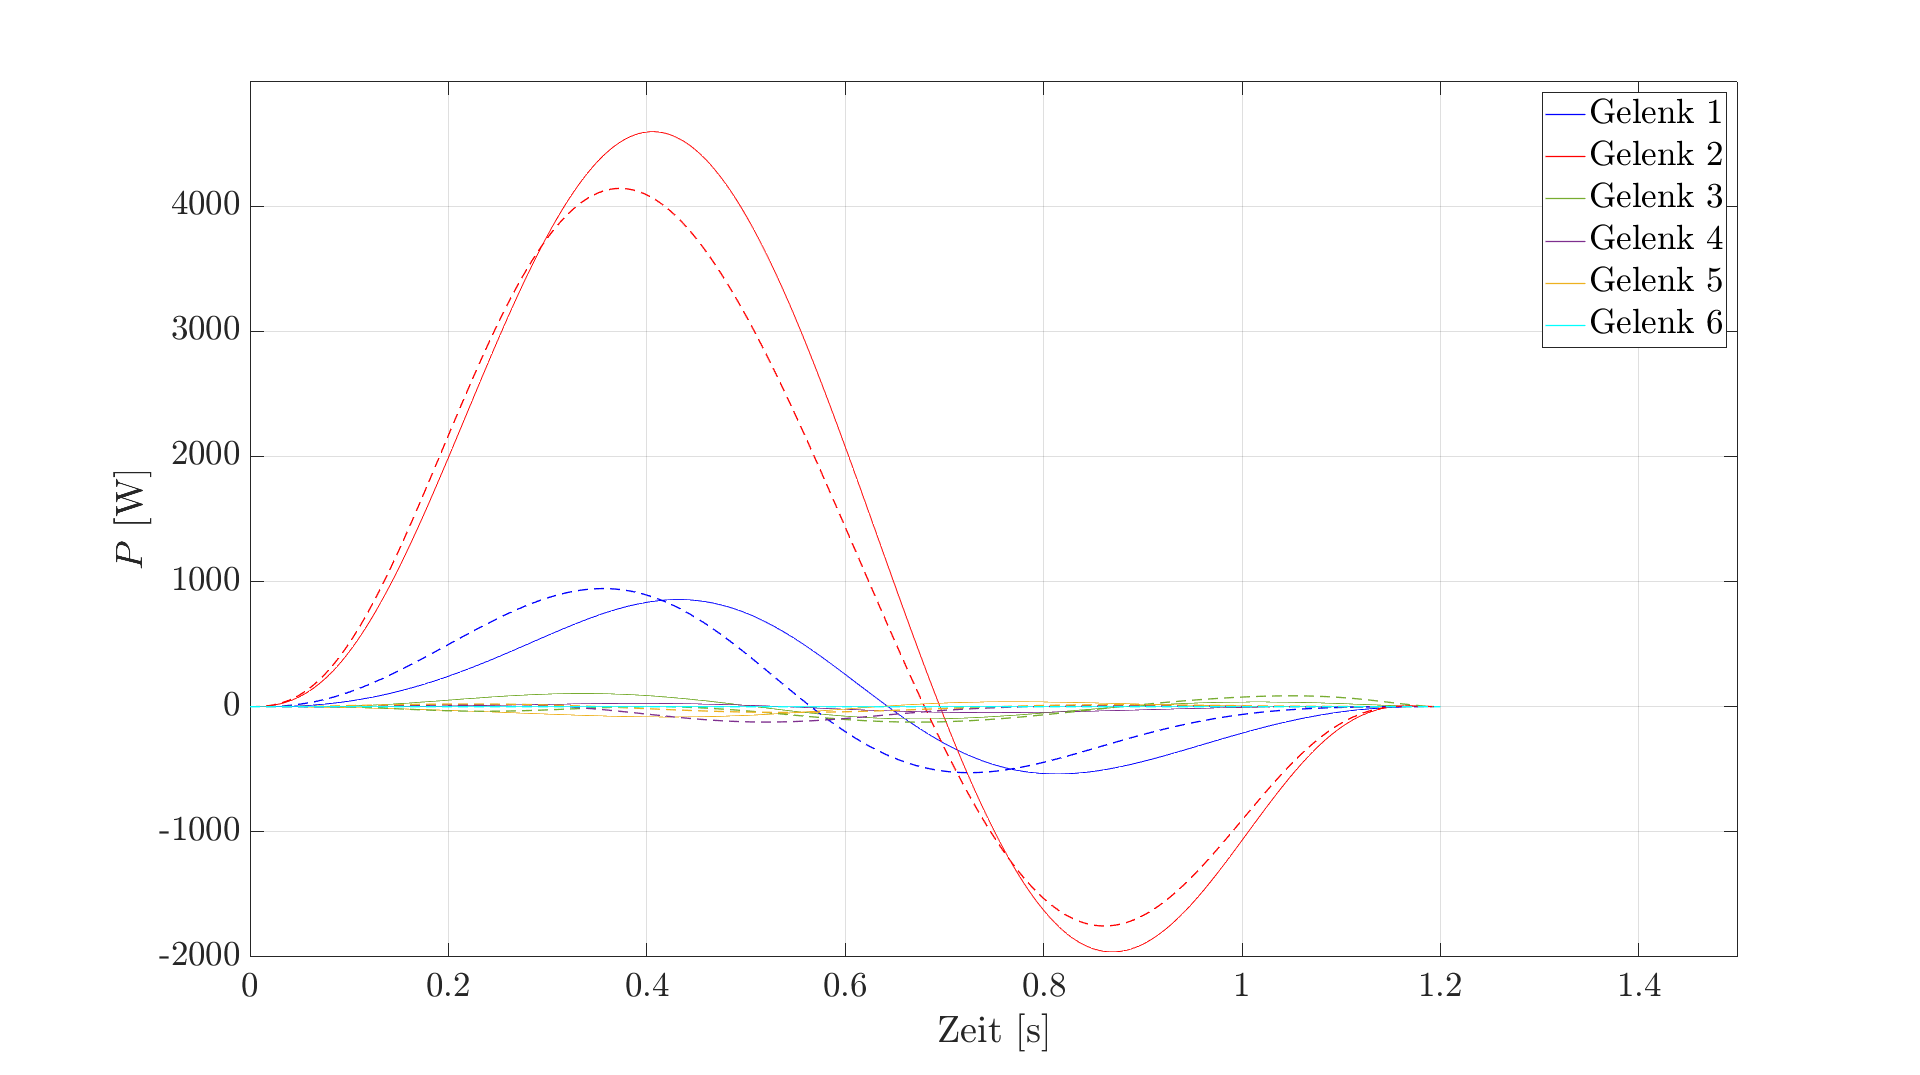
\includegraphics[width=1\linewidth]{images/Optimierungsergebnisse_up/popt}
	\caption{Simulierte Leistungsaufnahme der Initialbahn und optimierten Bewegungsbahn}
	\label{fig:popt}
\end{figure}
%
Nachfolgend werden die Geschwindigkeitsnebenbedingungen in Abbildung \ref{fig:velopt}sowie der Verlauf der Gelenkwinkel in Abbildung \ref{fig:posopt} untersucht. 
%
\begin{figure}[tbph]
	\centering
	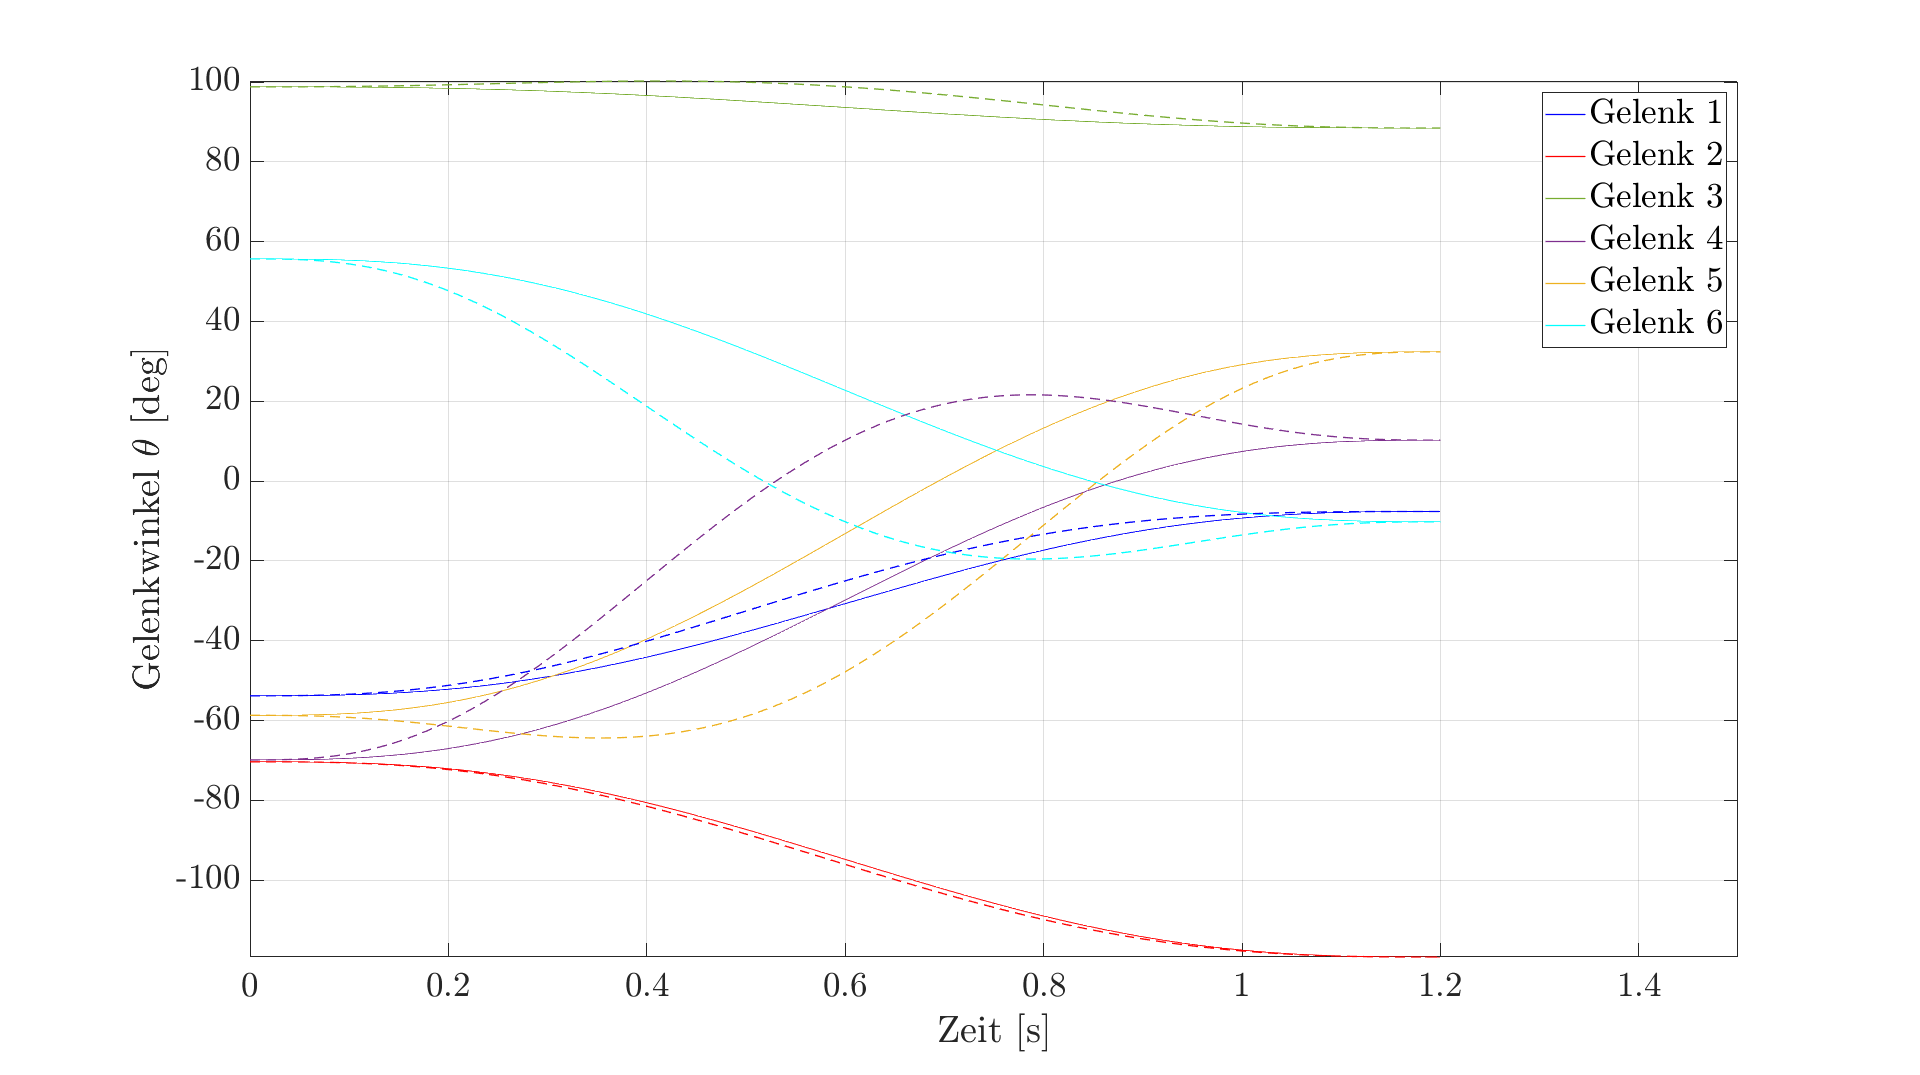
\includegraphics[width=1\linewidth]{images/Optimierungsergebnisse_up/posopt}
	\caption{Gelenkwinkelverläufe der Initialbahn und energieoptimierten Bewegungsbahn}
	\label{fig:posopt}
\end{figure}
%
\begin{figure}[tbph]
	\centering
	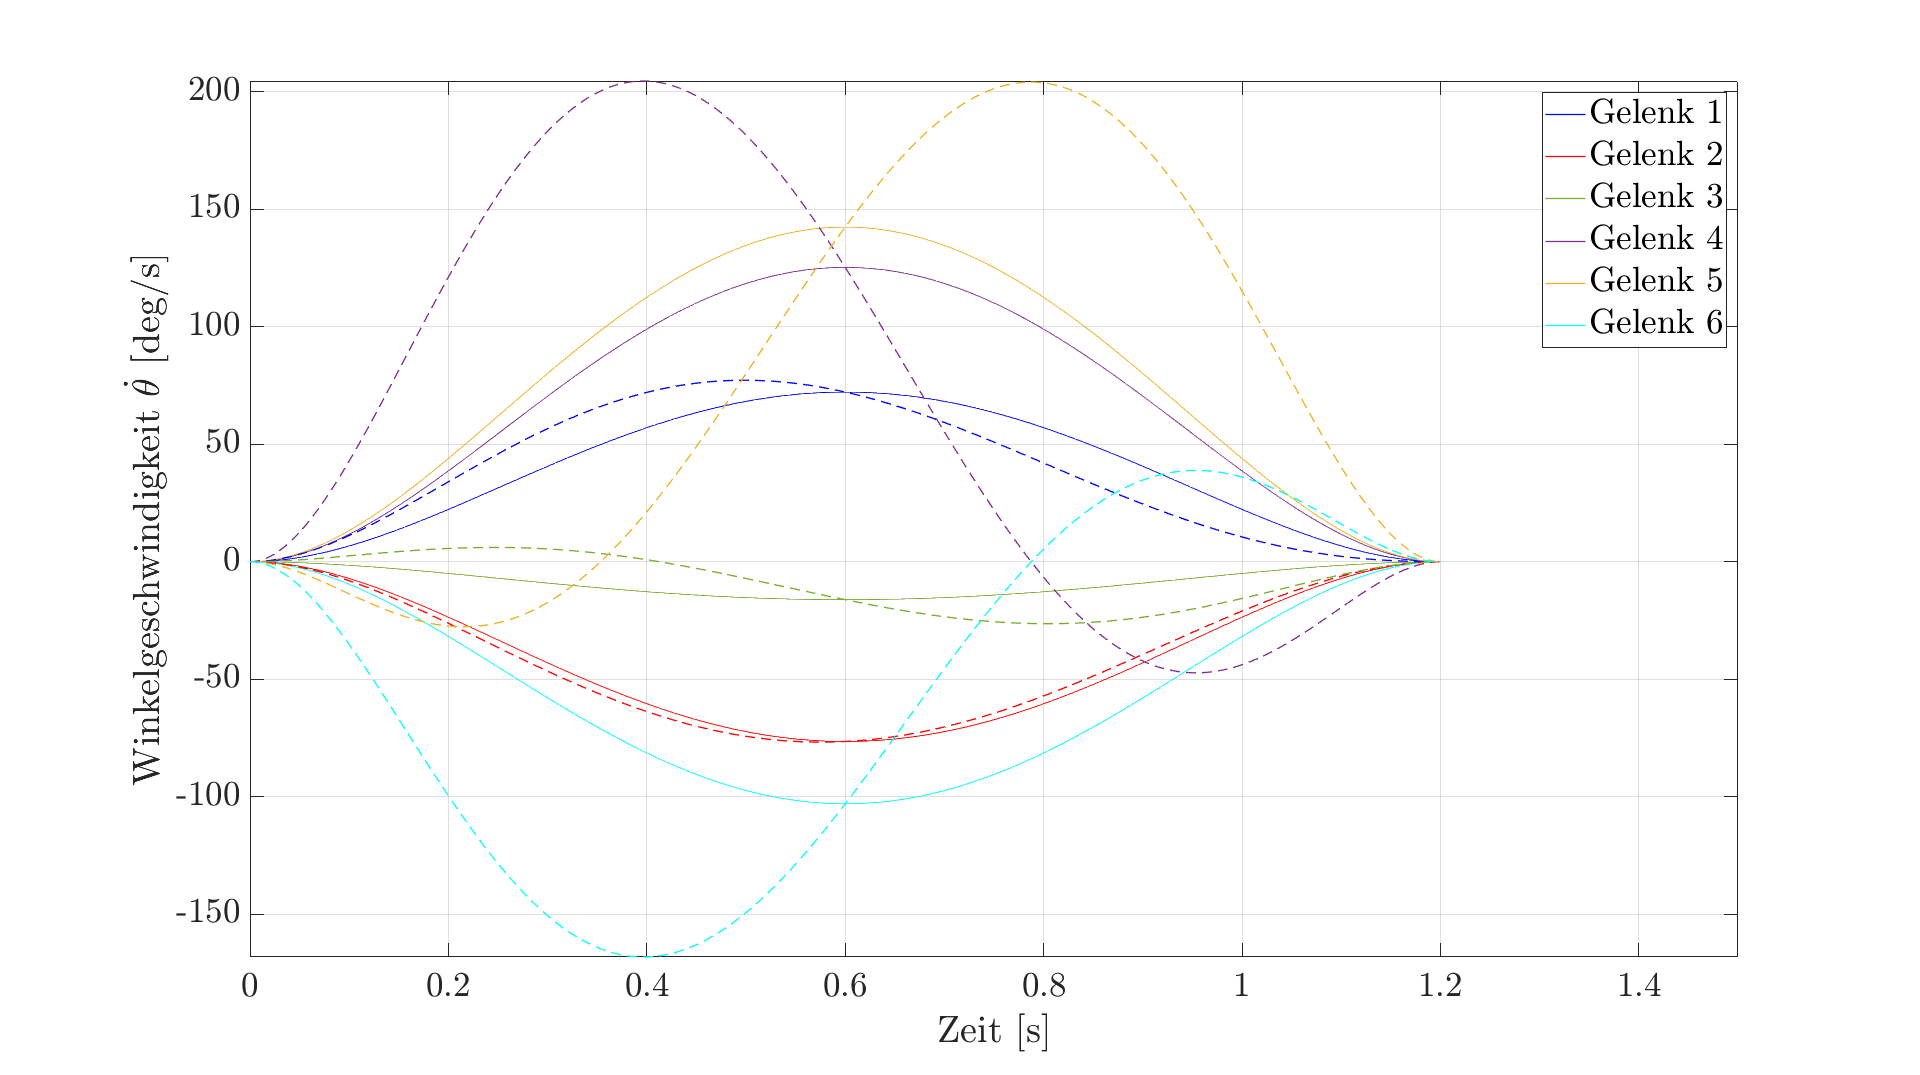
\includegraphics[width=1\linewidth]{images/Optimierungsergebnisse_up/velopt}
	\caption{Winkelgeschwindigkeitsverläufe der Initialbahn und energieoptimierten Bewegungsbahn}
	\label{fig:velopt}
\end{figure}
%
Für den Verlauf der Winkel im zweiten Gelenk sind keine auffälligen Abweichungen von der Initialbahn zu erkennen. Die beiden Verläufe der Gelenkwinkel eins und drei zeigen geringe Abweichungen im Bereich der Via-Punkte. Signifikante Unterschiede sind für die Verläufe der Gelenkwinkel vier, fünf und sechs erkennbar.  Bei Betrachtung der Abbildung \ref{fig:velopt} fällt auf, dass die Winkelgeschwindigkeiten $\dot{q}_{4}(t)$, $\dot{q}_{5}(t)$ und $\dot{q}_{6}(t)$ erheblich größer ausfallen als die Originalverläufe. Dies ist auf die Nähe der Gelenkwinkel ${q}_{v,4}$, ${q}_{v,5}$ und ${q}_{v,6}$ zu den Grenzwerten in Kombination mit der Größe des Gelenkwinkelhub $\Delta q_i = | q_{s,i}+q_{e,i} | ~\forall~ i \in \{4,5,6\}$ zurückzuführen. Infolgedessen werden die Via-Punkte ${q}_{v,4}$, ${q}_{v,5}$ und ${q}_{v,6}$ manuell auf den Mittelwert zwischen Initial-Via-Punkt und energieoptimalen Via-Punkt, siehe Gleichung \ref{eqn:manuellejustage} nachjustiert.
%
\begin{equation}
	\label{eqn:manuellejustage}
	{q}_{v,i,justiert} = \dfrac{{q}_{v,i,opt} + \dfrac{q_{s,i}+q_{e,i}}{2}}{2}~\forall~ i \in \{4,5,6\}
\end{equation}
%
Die resultierenden Winkelgeschwindigkeiten in Abbildung \ref{fig:veloptedit} und Winkelbeschleunigungen in Abbildung \ref{fig:accoptedit}  werden damit auf ein akzeptables Maß reduziert. Die energieoptimalen Verläufe sind gestrichelt, die justierten Verläufe gepunktet dargestellt.
%
\begin{figure}[tbph]
	\centering
	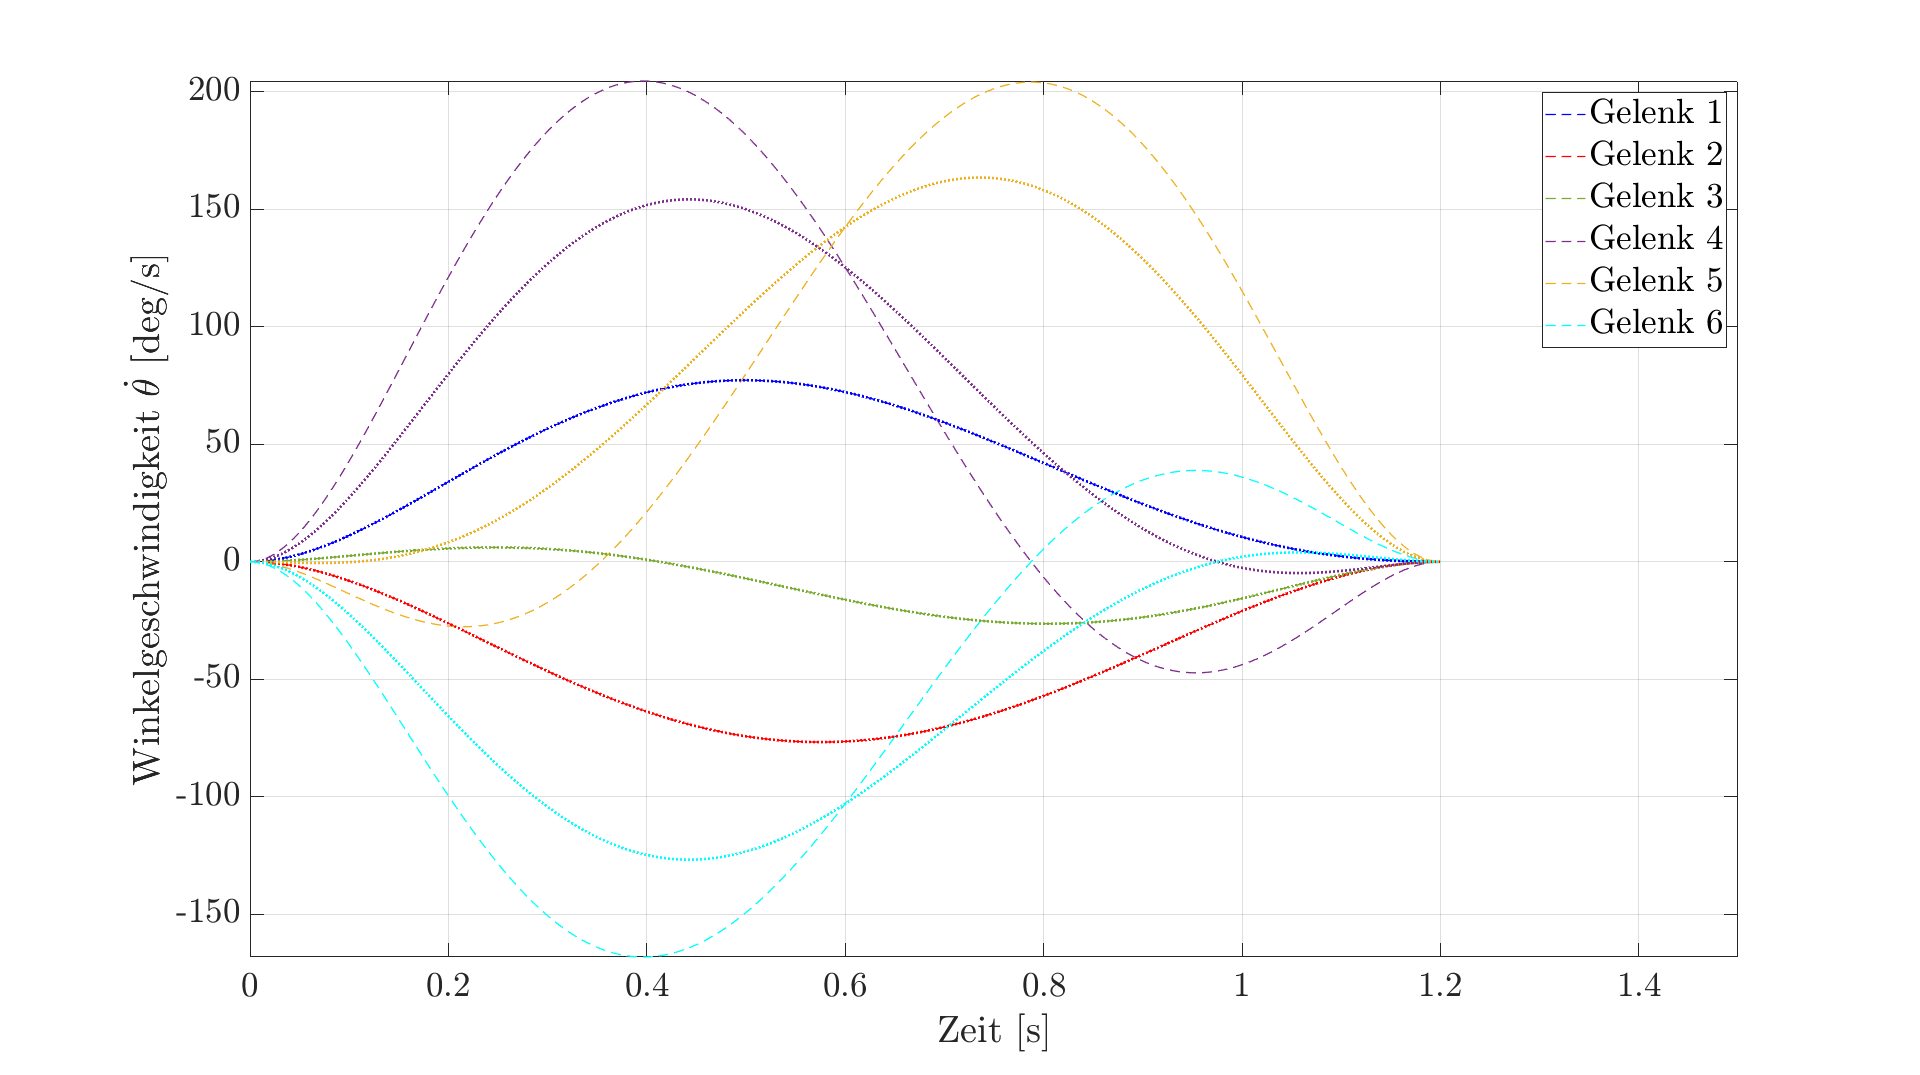
\includegraphics[width=1\linewidth]{images/Optimierungsergebnisse_up/veloptedit}
	\caption{Winkelgeschwindigkeitsverläufe der energieoptimierten Bewegungsbahn und justierten energieoptimierten Bewegungsbahn}
	\label{fig:veloptedit}
\end{figure}
%
\begin{figure}[tbph]
	\centering
	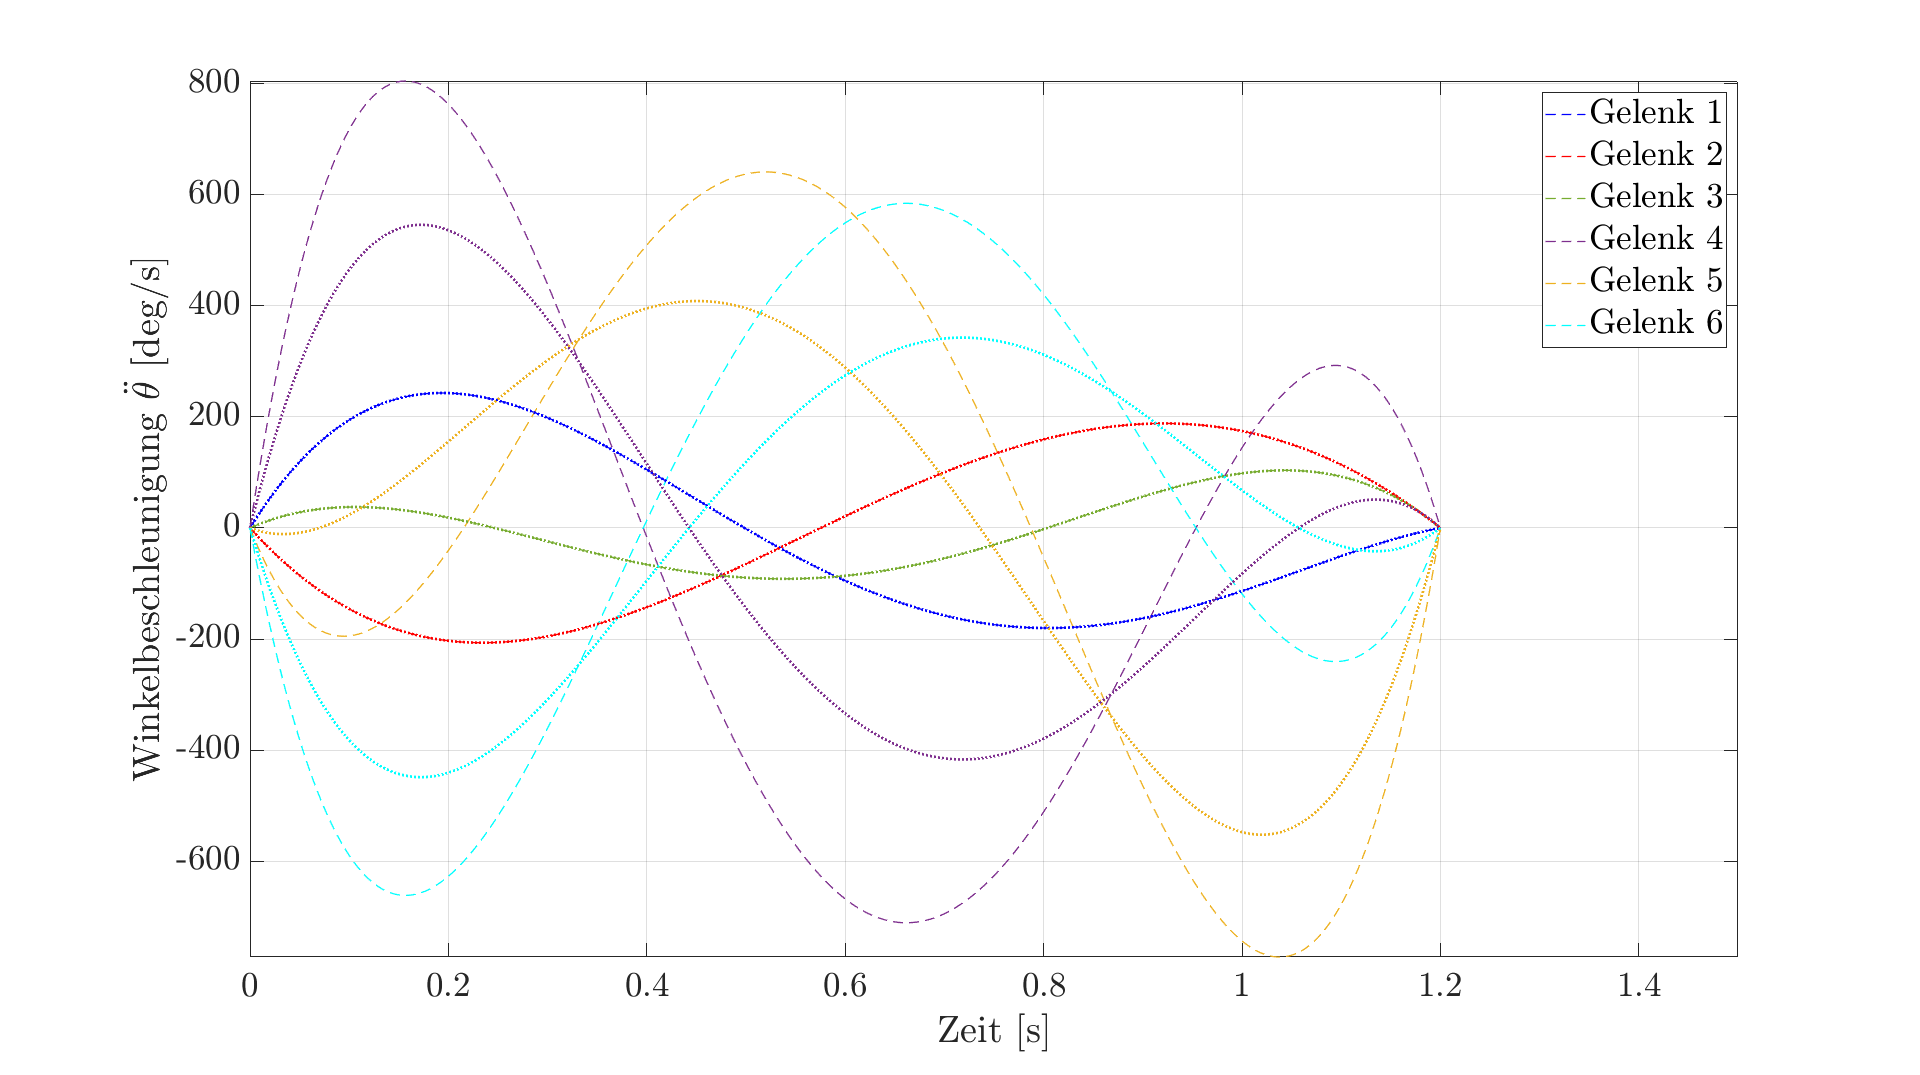
\includegraphics[width=1\linewidth]{images/Optimierungsergebnisse_up/accoptedit}
	\caption{Winkelbeschleunigungsverläufe der energieoptimierten Bewegungsbahn und justierten energieoptimierten Bewegungsbahn}
	\label{fig:accoptedit}
\end{figure}
%
Für den justierten Parametervektor beträgt der Energieverbrauch \textbf{1858 Joule} erzielt. Damit wird eine Energieeinsparung von 7,15 \% gegenüber der Initialbahn erzielt. Die Abbildungen für den Vergleich der initialen und justierten Verläufe aller relevanten Größen sind im Anhang \ref{acc:optupjust} aufgeführt.



\section{Validierung der Optimierungsergebnisse}
Ziel ist die Energieeinsparung auf Basis des optimierten Via-Punkts am realen System zu validieren. 
%
\subsection{Durchführung}
%Versuchsbeschreibung
%Definition von Start- und Zielpunkt
%Berechnung der Initialbahn durch die KR C
%Berechnung der Startviapunkte
\subsection{Auswertung}
%\begin{figure}[tbph]
%	\centering
%	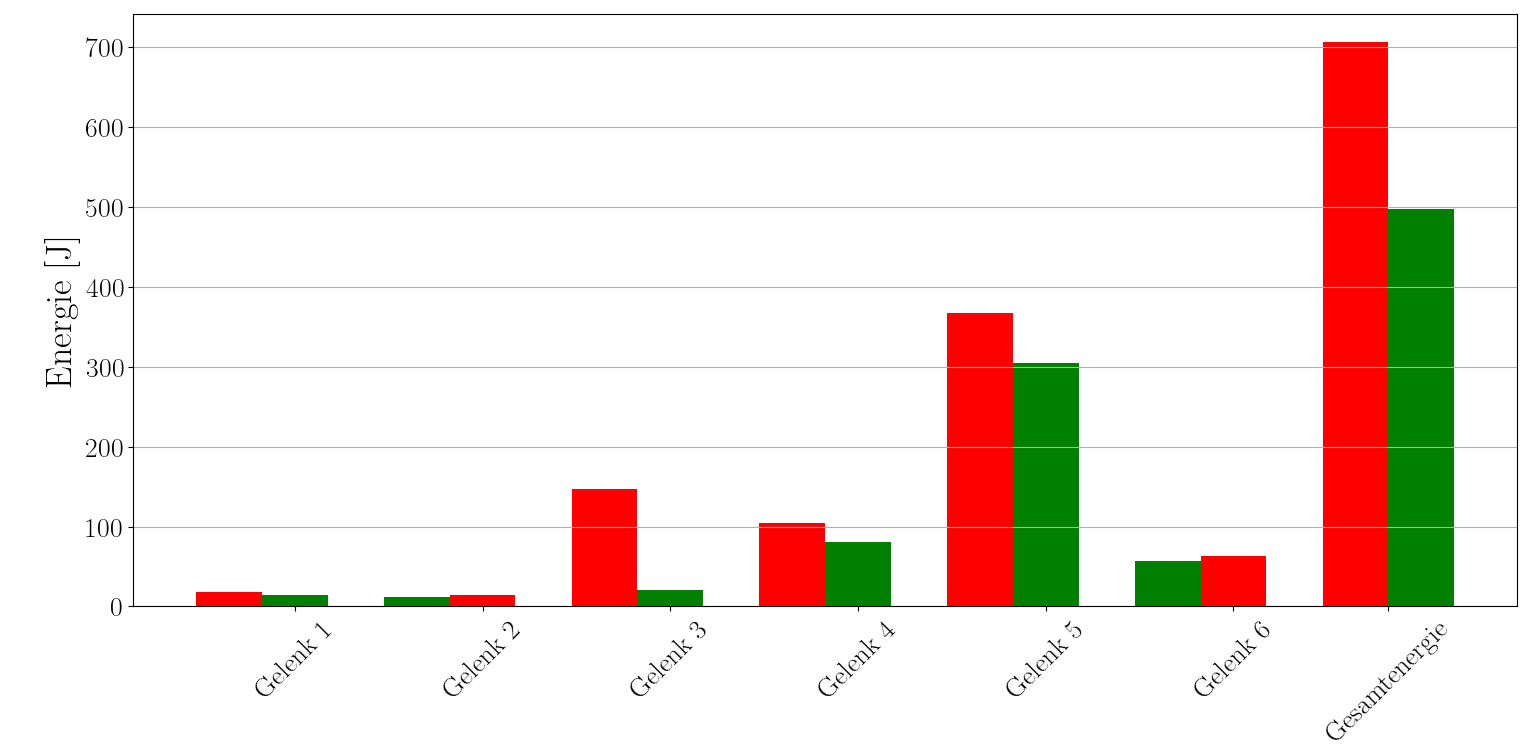
\includegraphics[width=1\linewidth]{images/e_down500}
%	\caption{Energieverbrauch Bewegung Eins}
%	\label{fig:edown500}
%\end{figure}
%\begin{figure}[tbph]
%	\centering
%	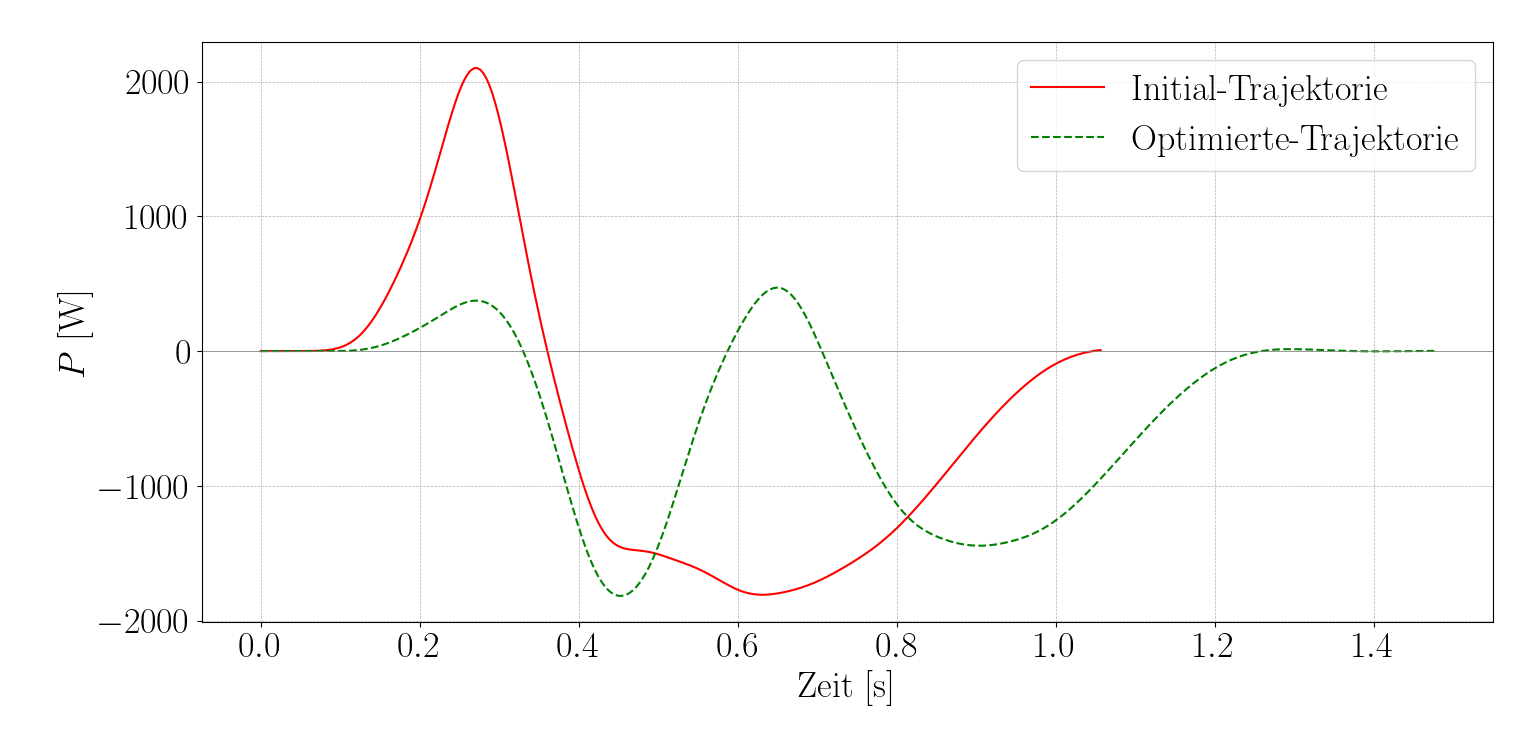
\includegraphics[width=1\linewidth]{images/P_down}
%	\caption{Leistungsaufnahme Bewegung Eins}
%	\label{fig:pdown}
%\end{figure}
%\begin{figure}[tbph]
%	\centering
%	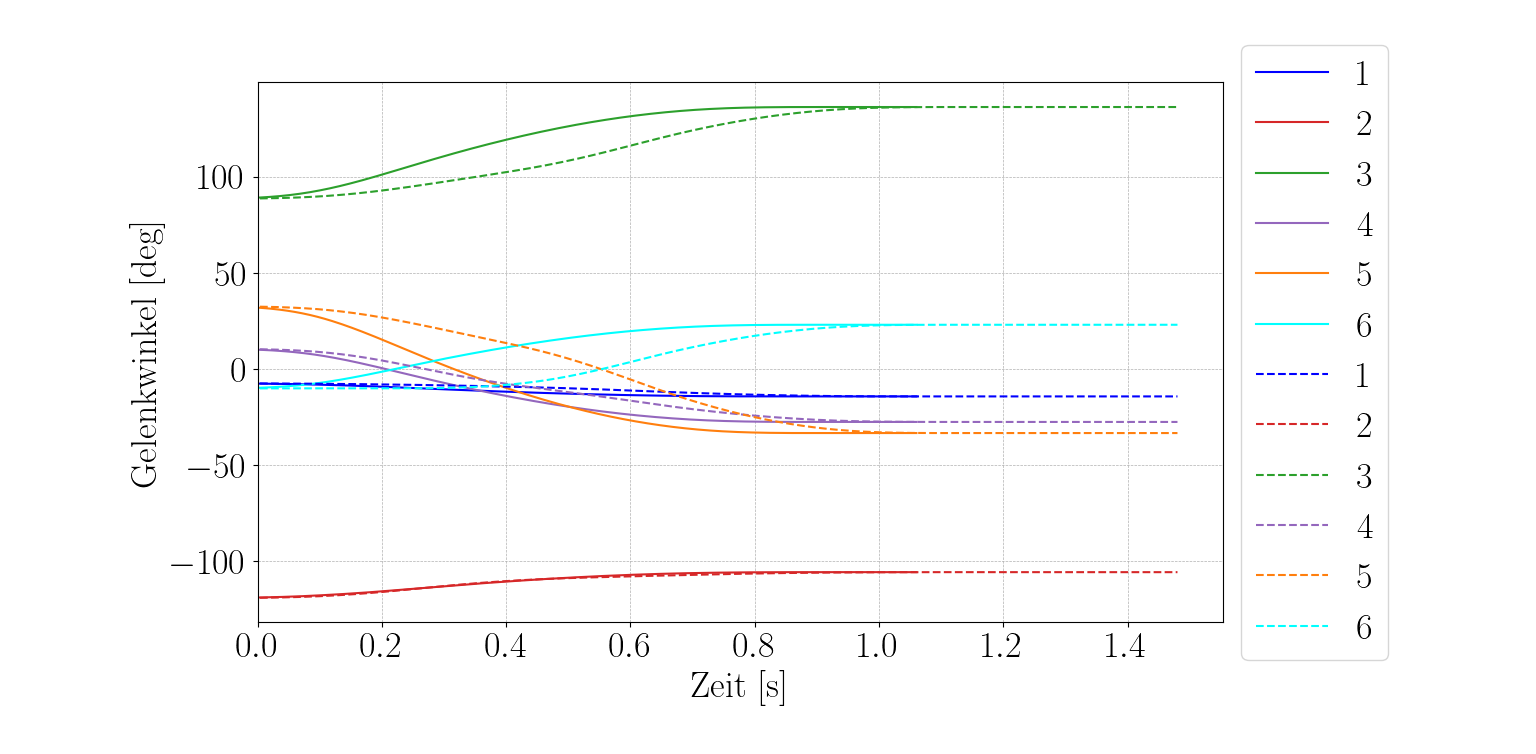
\includegraphics[width=1\linewidth]{images/aiposdown}
%	\caption{Gelenkwinkel Bewegung Eins}
%	\label{fig:aiposdown}
%\end{figure}
%\begin{figure}[tbph]
%	\centering
%	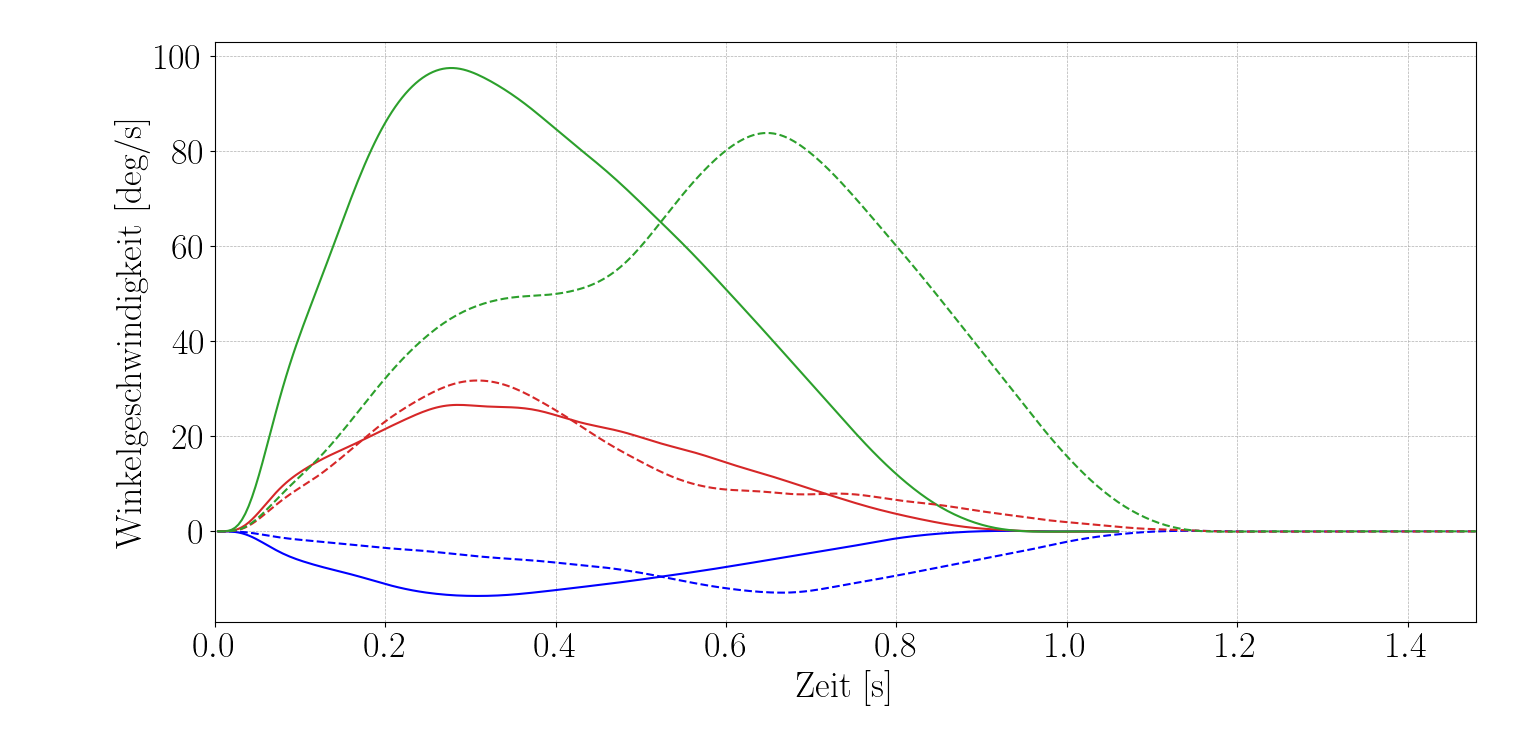
\includegraphics[width=1\linewidth]{images/velposdown1}
%	\caption{Winkelgeschwindigkeit in den Gelenken 1-3 Bewegung Eins}
%	\label{fig:velposdown1}
%\end{figure}
%\begin{figure}[tbph]
%	\centering
%	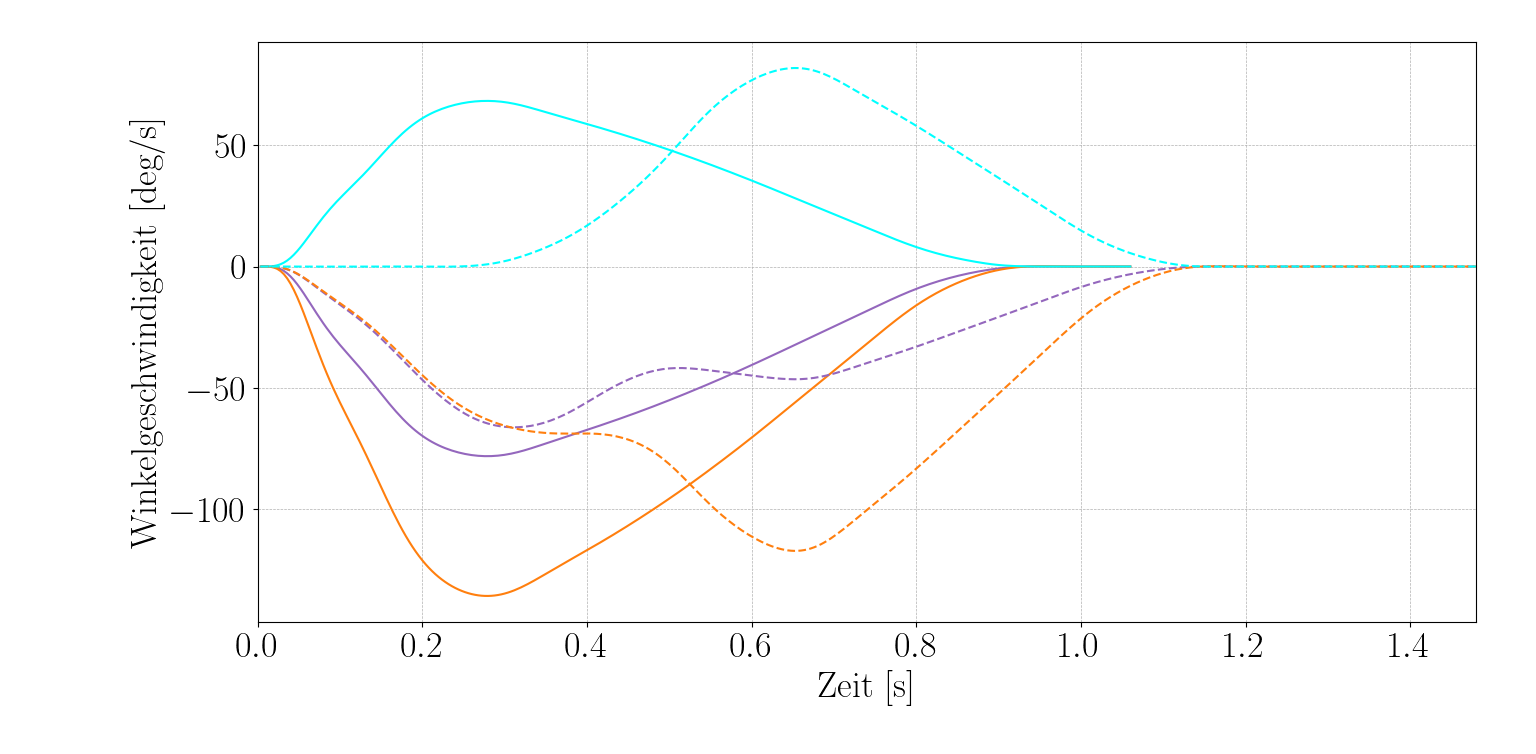
\includegraphics[width=1\linewidth]{images/velposdown2}
%	\caption{Winkelgeschwindigkeit in den Gelenken 4-6 Bewegung Eins}
%	\label{fig:velposdown2}
%\end{figure}
%\begin{figure}[tbph]
%	\centering
%	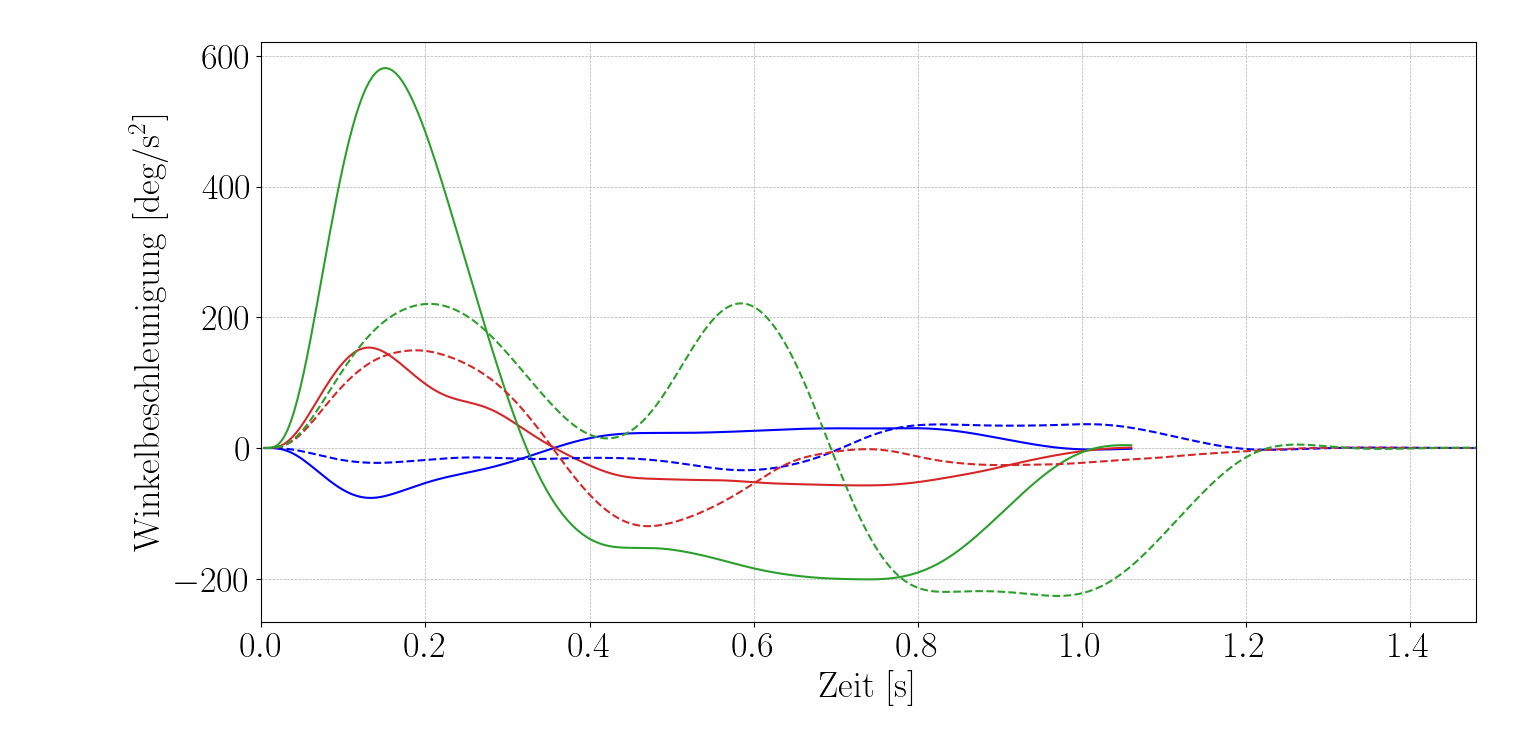
\includegraphics[width=1\linewidth]{images/accdown1}
%	\caption{Winkelbeschleunigung in den Gelenken 1-3 Bewegung Eins}
%	\label{fig:accdown1}
%\end{figure}
%\begin{figure}[tbph]
%	\centering
%	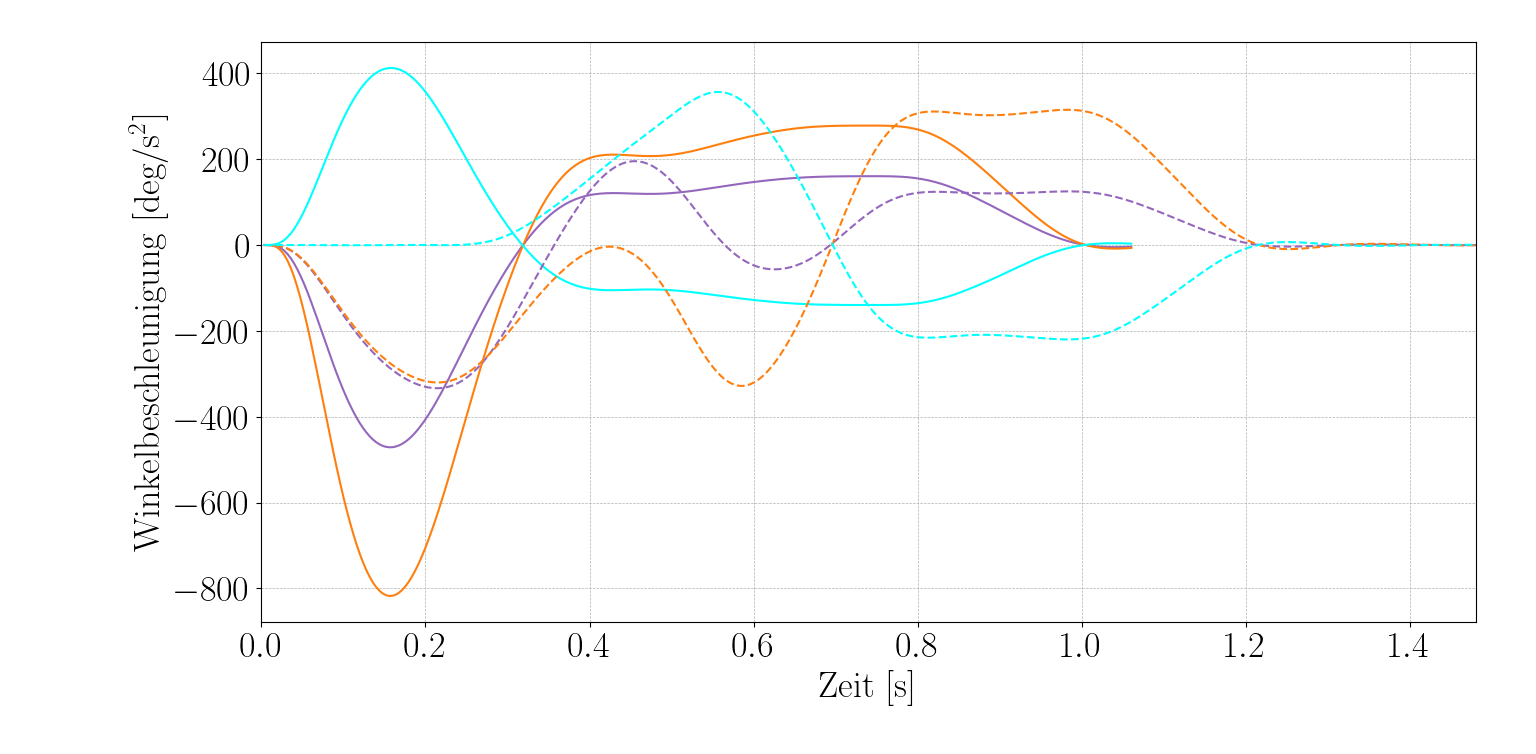
\includegraphics[width=1\linewidth]{images/accdown2}
%	\caption{Winkelbeschleunigung in den Gelenken 4-6 Bewegung Eins}
%	\label{fig:accdown2}
%\end{figure}
%
\begin{figure}[tbph]
	\centering
	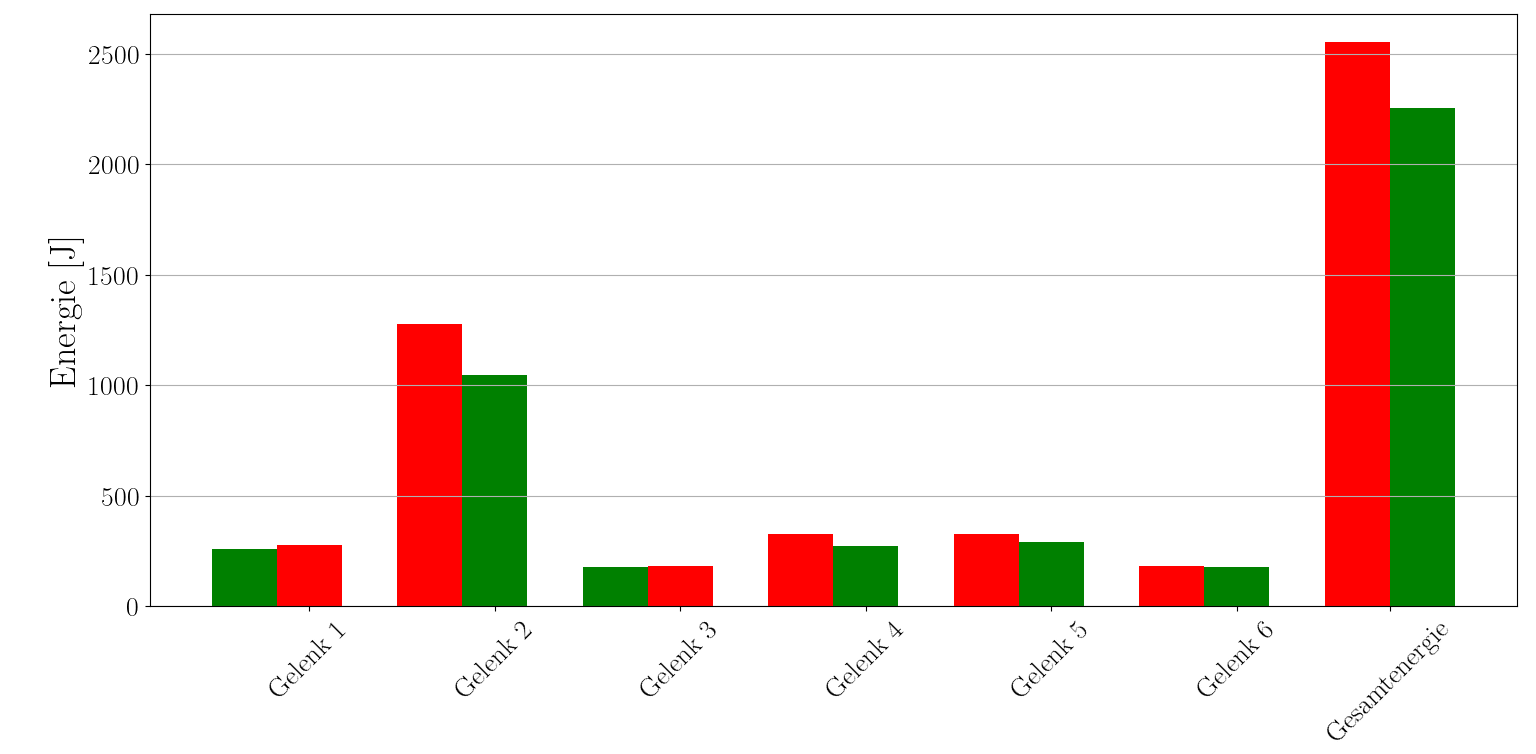
\includegraphics[width=1\linewidth]{images/e_up500}
	\caption{Energieverbrauch Bewegung Zwei}
	\label{fig:eup500}
\end{figure}
\begin{figure}[tbph]
	\centering
	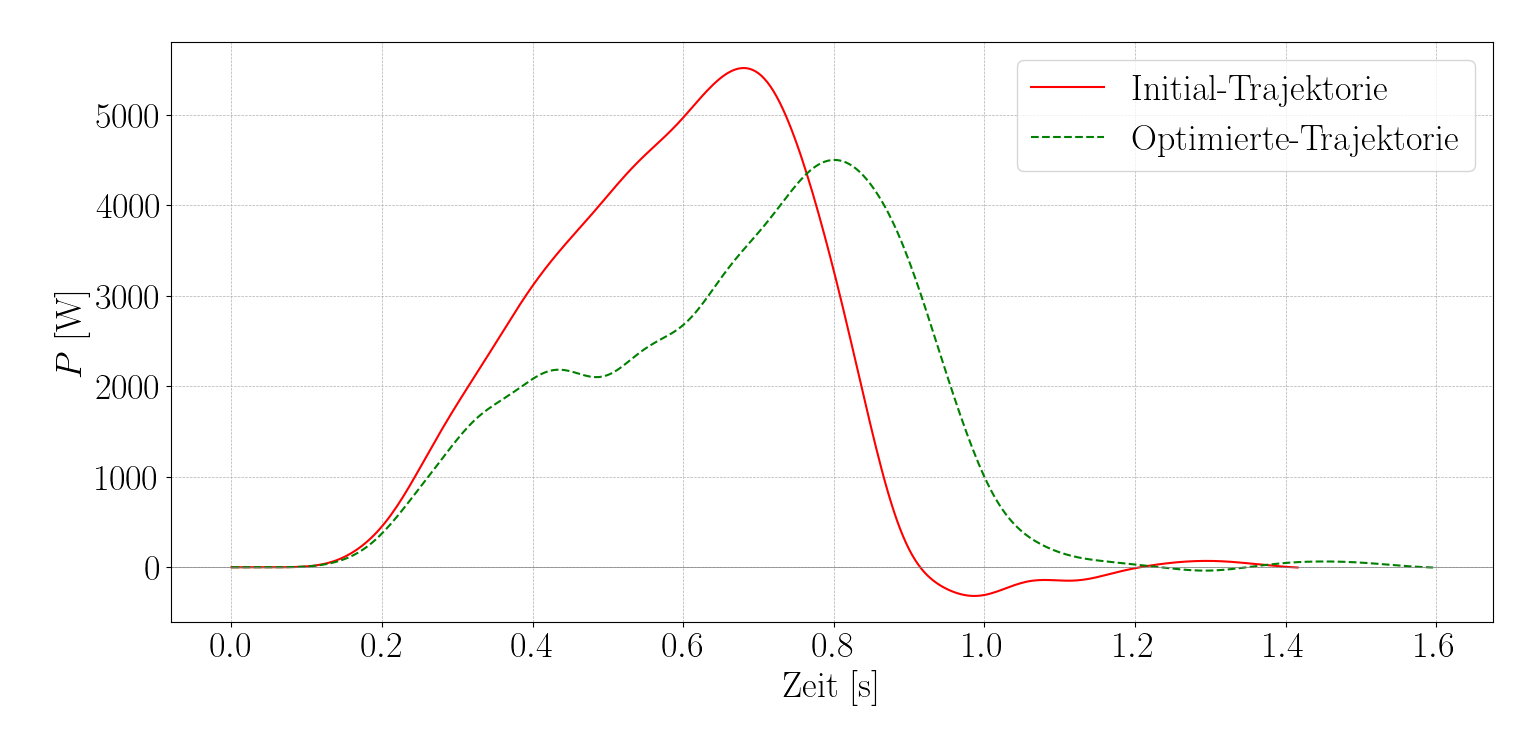
\includegraphics[width=1\linewidth]{images/P_up}
	\caption{Leistungsaufnahme Bewegung Zwei}
	\label{fig:pup}
\end{figure}
%\begin{figure}[tbph]
%	\centering
%	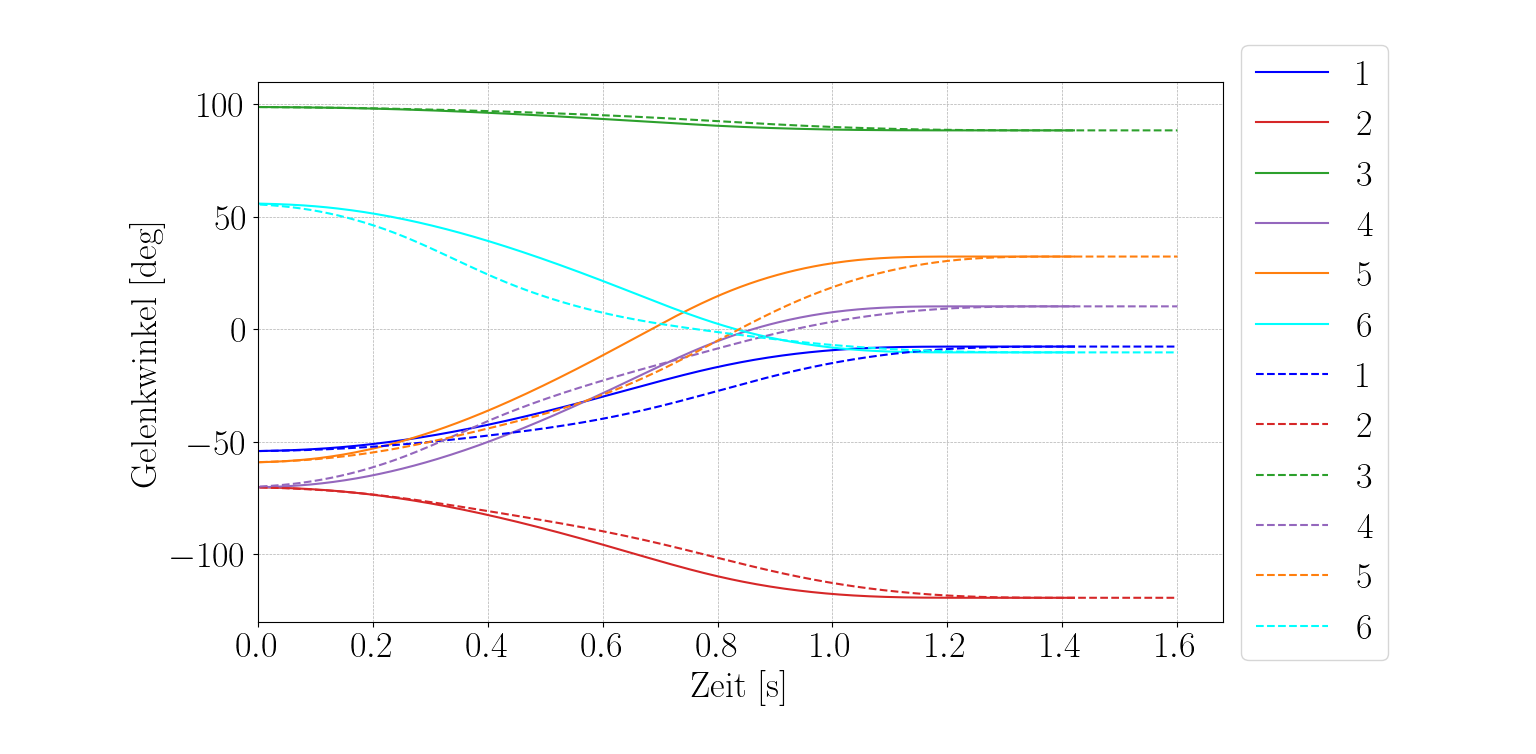
\includegraphics[width=1\linewidth]{images/aiposup}
%	\caption{Gelenkwinkel Bewegung Eins}
%	\label{fig:aiposup}
%\end{figure}
%\begin{figure}[tbph]
%	\centering
%	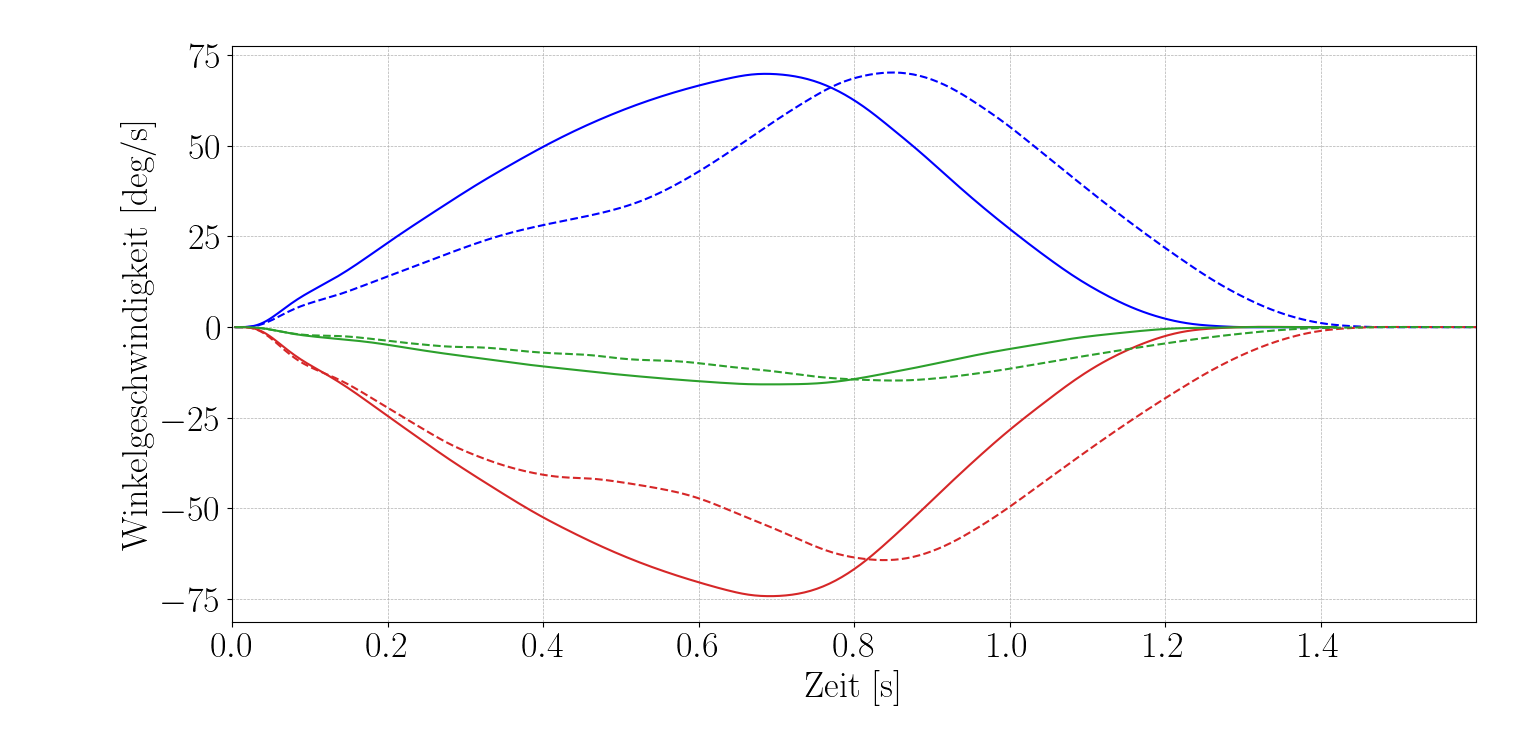
\includegraphics[width=1\linewidth]{images/velposup1}
%	\caption{Winkelgeschwindigkeit in den Gelenken 1-3 Bewegung Zwei}
%	\label{fig:velposup1}
%\end{figure}
%\begin{figure}[tbph]
%	\centering
%	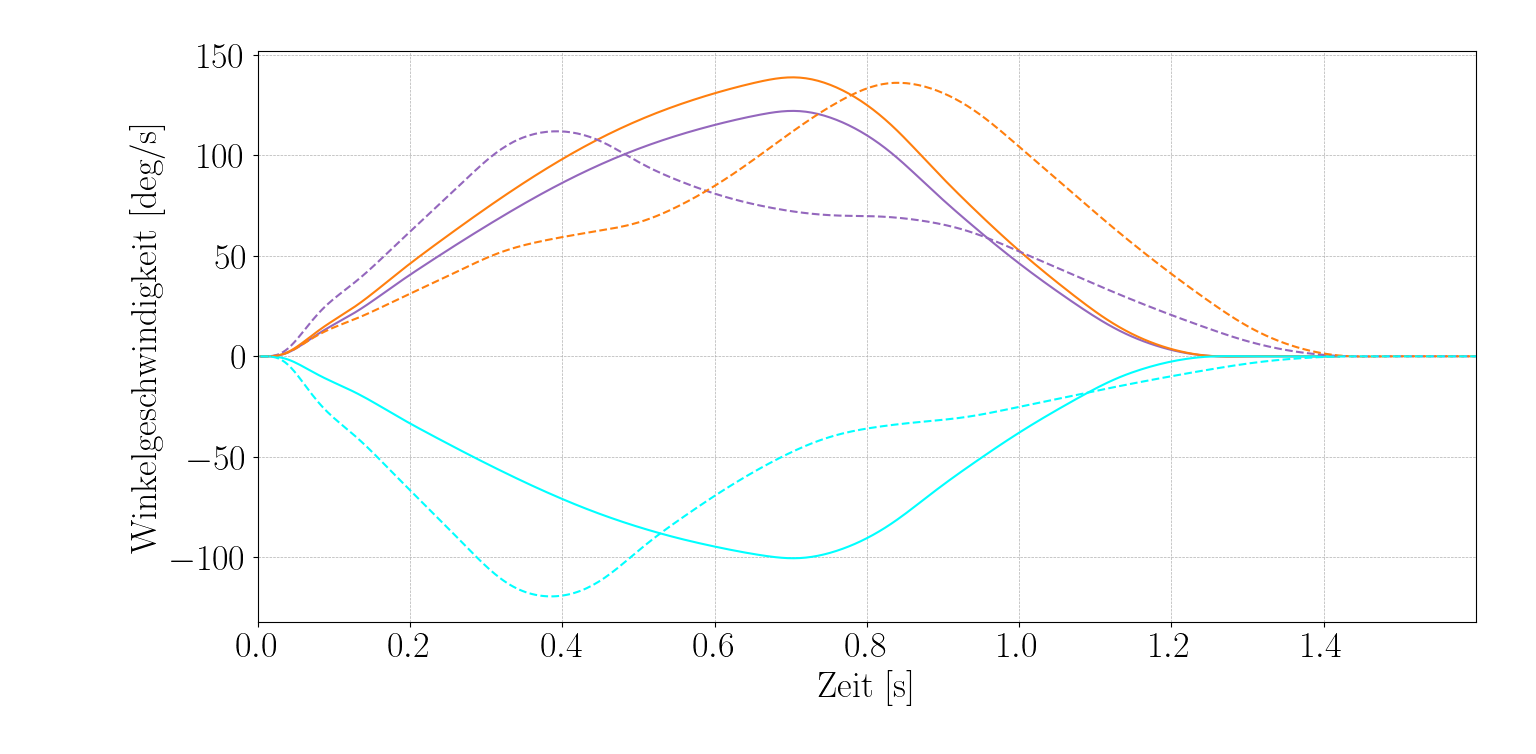
\includegraphics[width=1\linewidth]{images/velposup2}
%	\caption{Winkelgeschwindigkeit in den Gelenken 4-6 Bewegung Zwei}
%	\label{fig:velposup2}
%\end{figure}
%\begin{figure}[tbph]
%	\centering
%	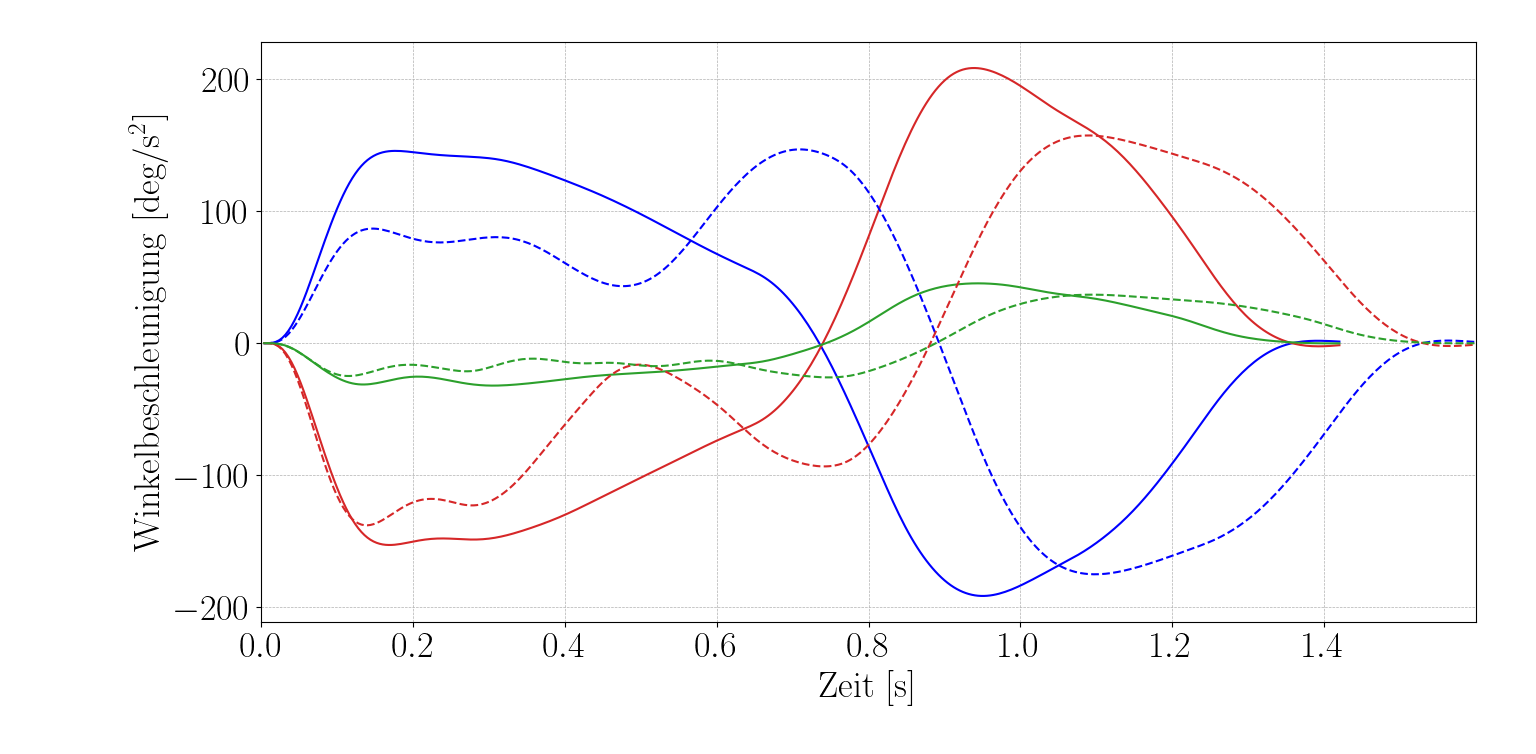
\includegraphics[width=1\linewidth]{images/accup1}
%	\caption{Winkelbeschleunigung in den Gelenken 1-3 Bewegung Zwei}
%	\label{fig:accup1}
%\end{figure}
%\begin{figure}[tbph]
%	\centering
%	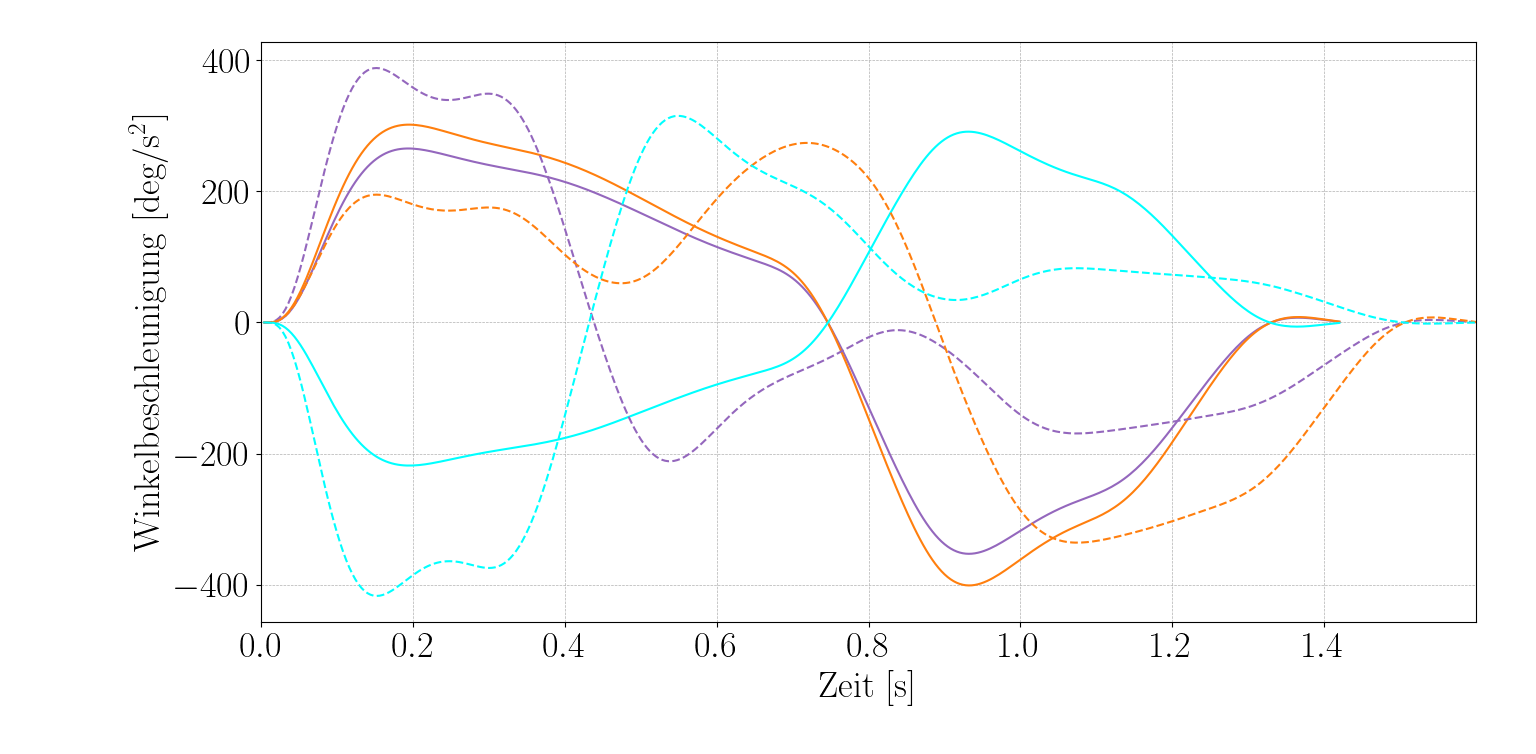
\includegraphics[width=1\linewidth]{images/accup2}
%	\caption{Winkelbeschleunigung in den Gelenken 4-6 Bewegung Zwei}
%	\label{fig:accup2}
%\end{figure}

\subsection{Schlussfolgerung} 

%

%\subsection{Fehlerquellen}
%Temperatureinfluss auf die Reibung 